\section{Technical Implementation Details}

This section outlines the core technologies and tools used in the development of the LiftDrop platform, along with key decisions regarding communication, backend logic, and system behavior.

\subsection{Technology Stack}

\begin{itemize}
    \item \textbf{Mobile Application}: Developed using Android Jetpack Compose (Kotlin), the app enables couriers to manage availability, respond to order requests, and track deliveries in real time.
    \item \textbf{Backend Server}: Built with Spring Web MVC, the server handles business logic, order assignment, session management, and serves RESTful and WebSocket endpoints.
    \item \textbf{Database}: PostgreSQL is used for structured data storage, including user profiles, order metadata, delivery history, and courier location logs.
    \item \textbf{Geospatial Services}: The Google Maps API is integrated to calculate distances, estimate travel times, and optimize courier-to-pickup assignment.
\end{itemize}

\subsection{Development Tools}

\begin{itemize}
    \item \textbf{Postman}: Used to test and validate REST endpoints during backend development.
    \item \textbf{Git and GitHub}: Used for version control, issue tracking, and collaborative development.
    \item \textbf{Android Studio}: The primary IDE for building and testing the Android application.
    \item \textbf{IntelliJ IDEA}: Used for backend development and debugging.
\end{itemize}

\subsection{Deployment Details}

\subsubsection{Backend Deployment}
The backend is hosted on Render, which automates building and deploying from a GitHub repository. On each push to the main branch, the application is rebuilt and restarted. Render manages horizontal scaling, environment variables, and secure HTTPS access.

\subsubsection{Database Hosting}
PostgreSQL is also managed by Render. Data is persisted in a cloud PostgreSQL instance, with automated backups enabled and access limited to the backend service.

\subsubsection{Environment Configuration}
Environment variables (e.g., API keys, DB connection URLs) are configured via the Render dashboard and injected during deployment.

\subsubsection{Security Considerations}
- HTTPS is enforced automatically by Render.
- Session cookies are marked HTTP-only and Secure.
- CORS is configured to restrict frontend access.

\subsubsection{Continuous Deployment}
Each push to the GitHub repository triggers an automatic build and deployment, ensuring that the most recent changes are reflected without manual intervention.


\subsection{Authentication and Authorization}

\subsubsection{Authentication}

To secure user sessions and API access, LiftDrop uses session-based authentication:

\begin{itemize}
    \item \textbf{HTTP-only Session Cookies}: Upon successful login, the backend generates a session cookie containing a signed token. The cookie is marked as HTTP-only, preventing JavaScript access and mitigating cross-site scripting (XSS) risks.
\end{itemize}

\subsubsection{Cookie Generation and Deletion}

The following Kotlin snippets show how the session cookie is generated and invalidated.

\begin{lstlisting}[language=Kotlin, caption={Generating the Session Cookie}]
ResponseCookie
    .from("auth_token", token)
    .path("/")
    .maxAge(Duration.ofDays(1))
    .httpOnly(true)
    .build()
\end{lstlisting}

\begin{lstlisting}[language=Kotlin, caption={Deleting the Session Cookie}]
ResponseCookie
    .from("auth_token", "")    // Clear the value
    .path("/")                 // Match the original path
    .maxAge(0)                 // Immediate expiry
    .httpOnly(true)
    .build()
\end{lstlisting}

\subsubsection{Authorization}

LiftDrop uses role-based access control (RBAC) to enforce feature access policies. Each API endpoint inspects the session token to determine whether the requester is a \texttt{Client} or a \texttt{Courier}. This is handled at the controller layer using a Spring \texttt{HandlerInterceptor}:

\begin{lstlisting}[language=Kotlin, caption={Condensed Kotlin-style pseudocode for AuthenticationInterceptor}]
@Component
class AuthenticationInterceptor(...) : HandlerInterceptor {
    override fun preHandle(request: HttpServletRequest, response: HttpServletResponse, handler: Any): Boolean {
        if (handler !is HandlerMethod) return true
        val authCookie = ... // extract auth cookie
        // Client auth (the same is done for the courier but with the AuthenticatedCourier class)
    if(handler.hasParameterType(AuthenticatedClient::class.java)){
            val client = authorizationHeaderProcessor.processClientAuthorizationHeaderValue(authCookie?.value)
            return client?.let {
    AuthenticatedClientArgumentResolver.addClientTo(it, request)
                true
            } ?: unauthorized(response) // returns false with a 401 status code
        } return true } }
\end{lstlisting}

This approach ensures that access is only granted to authenticated and properly authorized users based on their declared role. Unauthorized requests result in an HTTP \texttt{401 Unauthorized} response. It was made based on what was learned in the DAW course.

\subsection{Courier Location Updates}

Courier location tracking is implemented using Android \textbf{Foreground Services}, which allow the app to run and transmit location data even while running in the background.

To ensure efficient backend communication, the app retrieves the courier’s location every \textbf{30 seconds} but only transmits it under two conditions:
\begin{itemize}
    \item The courier is \textbf{logged in} and authenticated;
    %\item The courier has set their status to %\textbf{waiting for orders}.
\end{itemize}

Additionally, the system only sends a location update if the courier has moved more than \textbf{50 meters} since the last recorded position. This strategy minimizes unnecessary network traffic while maintaining sufficient tracking accuracy.

The 50-meter threshold was chosen based on common urban delivery speeds (e.g., 30~km/h for scooters or e-bikes), allowing meaningful movement to be captured without overwhelming the server. Furthermore, a delivery can only be confirmed if the courier is within 100 meters of the drop-off point—making the location filter both efficient and functionally sound.

\newpage

The simplified Kotlin pseudocode below outlines the core logic used for checking movement and conditionally sending location updates:

\begin{lstlisting}[language=Kotlin, caption={Condensed Kotlin-style pseudocode for Courier location updates mechanism}]
override fun startUpdating(authToken: String, courierId: String) {
    // Defines a high-accuracy location request every 30 seconds
    val request = LocationRequest.Builder(Priority.PRIORITY_HIGH_ACCURACY, 30_000L)
        .setMinUpdateIntervalMillis(30_000L).build()

    // Defines a callback to handle incoming location updates
    locationCallback = object : LocationCallback() {
        override fun onLocationResult(result: LocationResult) {
            val location = result.lastLocation ?: return

            // Launches coroutine to evaluate whether the update should be sent or not
            coroutineScope.launch {
                val movedEnough = lastSentLocation?.distanceTo(location)?.let { it > MIN_DISTANCE_METERS } != false
                if (movedEnough) {
                // Sends updated location to backend
                sendLocationToBackend(location.latitude, location.longitude, courierId, authToken)
                    lastSentLocation = location
                }
            }
        }
    }
    // Start location updates using the defined request and callback
    fusedLocationClient.requestLocationUpdates(request, locationCallback!!, Looper.getMainLooper())
}
\end{lstlisting}



\subsection{Communication Protocol}

The LiftDrop platform establishes real-time communication between couriers and the backend using a WebSocket connection. This channel supports continuous, bidirectional message exchange without the overhead of repeated HTTP requests.

Through this connection, the system manages key runtime events such as courier availability toggling, order assignment notifications, delivery status updates and cancellation handling.

All communication is structured as JSON messages and routed based on courier identity and session state. The backend keeps track of active connections, ensuring that messages are delivered only to the intended recipients. This approach guarantees low-latency synchronization during time-sensitive operations.

The following function demonstrates how a courier's acceptance of a delivery request is sent to the backend via WebSocket:

\vspace{5.0mm}

\begin{lstlisting}[language=Kotlin, 
  basicstyle=\ttfamily\small, 
  lineskip=-0.1pt,
  caption={Sending an acceptance message via WebSocket}]
override suspend fun acceptRequest(requestId: String, token: String): Boolean {
    val messageJson = """
        {
            "type": "DECISION",
            "requestId": "$requestId",
            "decision": "ACCEPT"
        }
    """.trimIndent()

    return webSocket?.send(messageJson) == true
}
\end{lstlisting}

\vspace{5.0mm}

On the backend, each incoming WebSocket message is parsed and routed according to its type. The server maintains a reference to the courier’s WebSocket session and invokes the corresponding handler based on the message status content. The snippet below illustrates the message dispatch logic:

\vspace{5.0mm}

\begin{lstlisting}[language=Kotlin, caption={Backend handling of incoming WebSocket messages}]
override fun handleTextMessage(
    session: WebSocketSession,
    message: TextMessage,
) {
    val json = jacksonObjectMapper().readTree(message.payload)
    when (json.get("type").asText()) {
        "DECISION"     -> handleCourierResponse(session, json)
        "READY", 
        "NOT_READY"    -> toggleCourierAvailability(session)
        else           -> println("Unknown message type")
    }
}
\end{lstlisting}

\subsubsection{WebSocket Configuration and Lifecycle}

LiftDrop uses Spring’s WebSocket support to manage real-time courier communication.

\textbf{Endpoint Registration:}  
The WebSocket endpoint is registered at \texttt{/ws/courier} via a configuration class \texttt{CourierWebSocketConfig}, which implements \texttt{WebSocketConfigurer}. The handler \texttt{CourierWebSocketHandler} is injected via constructor and manages all courier sessions. CORS is set to allow all origins for development (\texttt{setAllowedOrigins("*")}).

\newpage

\textbf{Handler Role:}  
\texttt{CourierWebSocketHandler} extends \texttt{TextWebSocketHandler} and is responsible for:
\begin{itemize}
    \item Maintaining active courier sessions.
    \item Routing messages like \texttt{READY}, \texttt{DECISION}, and cancellations.
    \item Broadcasting updates to relevant connected users.
\end{itemize}

\textbf{Use Cases:}
\begin{itemize}
    \item Order assignment and courier responses.
    \item Availability toggling.
    \item Live updates on delivery status.
\end{itemize}

\subsection{Error Handling}

To ensure robustness and clarity in the face of runtime failures, LiftDrop adopts a layered error-handling strategy. This architecture supports clear diagnostics, consistent logging, user-oriented feedback, and modular server behavior—principles influenced by best practices studied in the DAW course.

\subsubsection{Result Modeling with \texttt{Either}}

Internally, success and failure outcomes are represented using a functional-style result type:

\begin{lstlisting}[language=Kotlin, caption={Functional Result Modeling with Either}]
sealed class Either<out L, out R> {
    data class Left<out L>(val value: L) : Either<L, Nothing>()
    data class Right<out R>(val value: R) : Either<Nothing, R>()
}

fun <R> success(value: R) = Either.Right(value)
fun <L> failure(error: L) = Either.Left(error)
\end{lstlisting}

This model ensures that failure handling is explicit and composable, improving testability and reducing reliance on exceptions.

\newpage

\subsubsection{Standardized API Errors with Problem Details}

For all HTTP interactions, the backend follows the \textbf{RFC 7807 Problem Details for HTTP APIs} specification. This standard defines a JSON structure for expressing errors in a machine-readable way:

\begin{lstlisting}[language=Kotlin, caption={Problem Details Model}]
data class Problem(
    val type: String?,
    val title: String?,
    val status: Int?,
    val detail: String?,
    val instance: String? = null
)
\end{lstlisting}

Responses use the \texttt{application/problem+json} media type and include fields such as \texttt{status}, \texttt{title}, and \texttt{detail} to clearly describe what went wrong.

A centralized factory exposes named constructors like:
\begin{itemize}
  \item \texttt{courierNotNearPickup()}
  \item \texttt{ratingAlreadyDone()}
  \item \texttt{userAlreadyExists()}
  \item \texttt{invalidRequestContent()}
\end{itemize}

Each problem type links to documentation hosted at:

\texttt{https://github.com/isel-sw-projects/2025-lift-drop/tree/main/docs/problems}

\subsubsection{Global Exception Handling}

All errors not handled by business logic are intercepted by a custom Spring \texttt{@ControllerAdvice}, shown below:

\begin{lstlisting}[language=Kotlin, caption={Global Exception Handler}]
@ControllerAdvice
class CustomExceptionHandler : ResponseEntityExceptionHandler() {

    override fun handleMethodArgumentNotValid(...) =
        Problem.invalidRequestContent("Argument received is not valid")
               .response(HttpStatus.BAD_REQUEST)

    override fun handleTypeMismatch(...) =
        Problem.invalidRequestContent("There is a type mismatch")
               .response(HttpStatus.BAD_REQUEST)


    
    override fun handleHttpMessageNotReadable(...) =
        Problem.invalidRequestContent("Http message is not readable")
               .response(HttpStatus.BAD_REQUEST)

    @ExceptionHandler(Exception::class)
    fun handleAllExceptions(ex: Exception, request: WebRequest): ResponseEntity<String> {
        GlobalLogger.log("Http.CustomExceptionHandler AllExceptions: $ex")
        return ResponseEntity.status(HttpStatus.INTERNAL_SERVER_ERROR)
                             .body("Internal Server Error")
    }
}
\end{lstlisting}

This handler ensures:
\begin{itemize}
    \item Graceful fallback for unexpected issues.
    \item Logged diagnostics.
    \item Consistent error responses for clients.
\end{itemize}

\subsubsection{Frontend Feedback Integration}

Errors returned in \texttt{Problem} format are parsed and used in the Android application to display appropriate UI feedback (e.g., invalid login, wrong pickup code, courier not near drop-off).


\newpage

\subsection{Frontend State Management}

\subsubsection{Message Handling and State Updates}

The LiftDrop mobile application adopts a reactive UI architecture using Jetpack Compose, where screen behavior is driven by immutable state objects. This approach ensures consistent rendering and predictable transitions throughout the user experience. Each screen is modeled using a dedicated sealed class that encapsulates its possible UI states. The use of state-driven design and reactive patterns in the development of the application was informed by concepts learned in the PDM course.

For example, the login and registration processes are controlled by the \texttt{LoginScreenState} and \texttt{RegisterScreenState} classes, respectively. These include the following variants:

\begin{description}
    \item[LoginScreenState:] \texttt{Idle}, \texttt{Login}, \texttt{Error}
    \item[RegisterScreenState:] \texttt{Idle}, \texttt{Register}, \texttt{Error}
\end{description}

These states allow the UI to reflect user progress during authentication, including success and failure outcomes.

The Home screen follows a more complex state model, represented by the sealed class \texttt{HomeScreenState}. The simplified listing below outlines all defined UI states used throughout the delivery lifecycle—including request reception, pickup, drop-off, cancellation, and confirmation.

\begin{lstlisting}[language=Kotlin, caption={Simplified HomeScreenState sealed class}]
sealed class HomeScreenState {
    data class Listening(...) : HomeScreenState()
    data class RequestAccepted(...) : HomeScreenState()
    data class RequestDeclined(...) : HomeScreenState()
    data class HeadingToPickUp(...) : HomeScreenState()
    data class PickedUp(...) : HomeScreenState()
    data class HeadingToDropOff(...) : HomeScreenState()
    data class Delivered(...) : HomeScreenState()
    data class Idle(...) : HomeScreenState()
    data class Error(...) : HomeScreenState()
    data class Logout(...) : HomeScreenState()
    data class CancellingOrder(...) : HomeScreenState()
    data class CancellingPickup(...) : HomeScreenState()
    data class CancellingDropOff(...) : HomeScreenState()
}
\end{lstlisting}

All screen states are managed using a \texttt{StateFlow} in the ViewModel layer. When updates are received—either from real-time WebSocket messages or local UI interactions— the corresponding ViewModel processes the event and updates the screen state accordingly. These updates propagate automatically to composables, ensuring reactive rendering and a consistent, unidirectional data flow throughout the application.

Error handling is also integrated into the state model. Whenever an unexpected event occurs—such as receiving a malformed message or encountering a failure while listening for updates—the ViewModel updates the state to \texttt{HomeScreenState.Error}. The UI reacts accordingly, displaying contextual information to the user, such as the problem title and message, to clearly indicate what went wrong.
To better illustrate how the error state appears in practice, Figure 11 shows the application’s response when a delivery fails mid-process.

\begin{figure}[H]
    \centering
    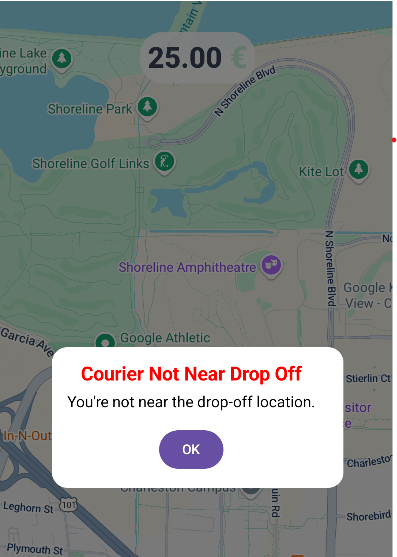
\includegraphics[width=0.44\textwidth]{images/ErrorScreenState.png}
    \caption{Error screen state when delivering order}
    \label{fig:incoming-request-screen}
\end{figure}

\newpage

The following example illustrates how the Home screen begins listening for messages and updates its state based on the received input:

\begin{lstlisting}[language=Kotlin, caption={Simplified WebSocket message handling in startListening}]
fun startListening() {
    viewModelScope.launch {
        val token = ... // Retrieved from DataStore
        homeService.startListening(
            token = token,
            onMessage = { msg ->
                when (val req = parseDynamicMessage(msg)) {
                    is IncomingRequestDetails -> _stateFlow.update { processIncomingRequest(it, req) }
                    is DeliveryUpdate         -> _stateFlow.update { processDeliveryUpdate(it, req) }
                    is ResultMessage          -> _stateFlow.update { processResultMessage(it, req) }
                    else                      -> ...
                }
            },
            onFailure = { _stateFlow.update { ... } }
        )
        _stateFlow.update { ... } // Initialize to Listening state
    }
}
\end{lstlisting}


Incoming WebSocket messages are sent in a unified JSON format and differentiated by a \texttt{type} field. The \texttt{parseDynamicMessage} function reads this field and dynamically maps the message to its corresponding class using Jackson. This pattern supports extensibility and ensures that each message type is handled appropriately in the ViewModel:

\begin{lstlisting}[language=Kotlin, caption={Dynamically parsing incoming WebSocket messages}]
fun parseDynamicMessage(message: String): HomeMessage {
    val mapper = jacksonObjectMapper()
    val root: JsonNode = mapper.readTree(message)
    val typeValue = root.get("type")?.asText() 
        ?: throw IllegalArgumentException("Missing type field")

    val type = MessageType.fromValue(typeValue) 
        ?: throw IllegalArgumentException("Unknown message type: $typeValue")

    return when (type) {
        MessageType.DELIVERY_REQUEST -> 
            mapper.treeToValue(root, IncomingRequestDetails::class.java)
        MessageType.DELIVERY_UPDATE -> 
            mapper.treeToValue(root, DeliveryUpdate::class.java)
        MessageType.SUCCESS, MessageType.ERROR -> 
            mapper.treeToValue(root, ResultMessage::class.java)
    }
}
\end{lstlisting}

The following diagram provides a high-level overview of a complete delivery request assignment cycle, illustrating how messages are exchanged between the backend and the courier application via WebSocket. It captures the progression from the initial assignment message to the courier's decision and the backend's final acknowledgment, all of which contribute to state transitions within the application.


\begin{figure}[H]
    \centering
    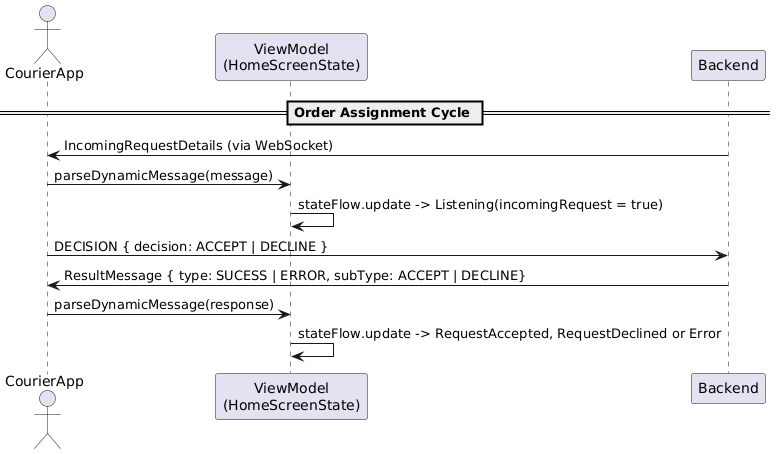
\includegraphics[width=0.85\textwidth]{images/MessageExchangeExample.png}
    \caption{Message exchange between backend and frontend during a delivery request cycle}
    \label{fig:message-sequence}
\end{figure}

Before heading to either the pickup or drop-off location, couriers are prompted to choose their preferred navigation application. Instead of enforcing a default, LiftDrop uses Android's intent system to display a list of compatible apps installed on the device—such as Google Maps, Waze, or other mapping tools. Once the courier selects an app, it is launched with the appropriate destination coordinates already filled in.

\newpage

The user interface mirrors this flow as illustrated below:

\begin{figure}[H]
    \centering
    \begin{subfigure}[b]{0.48\textwidth}
        \centering
        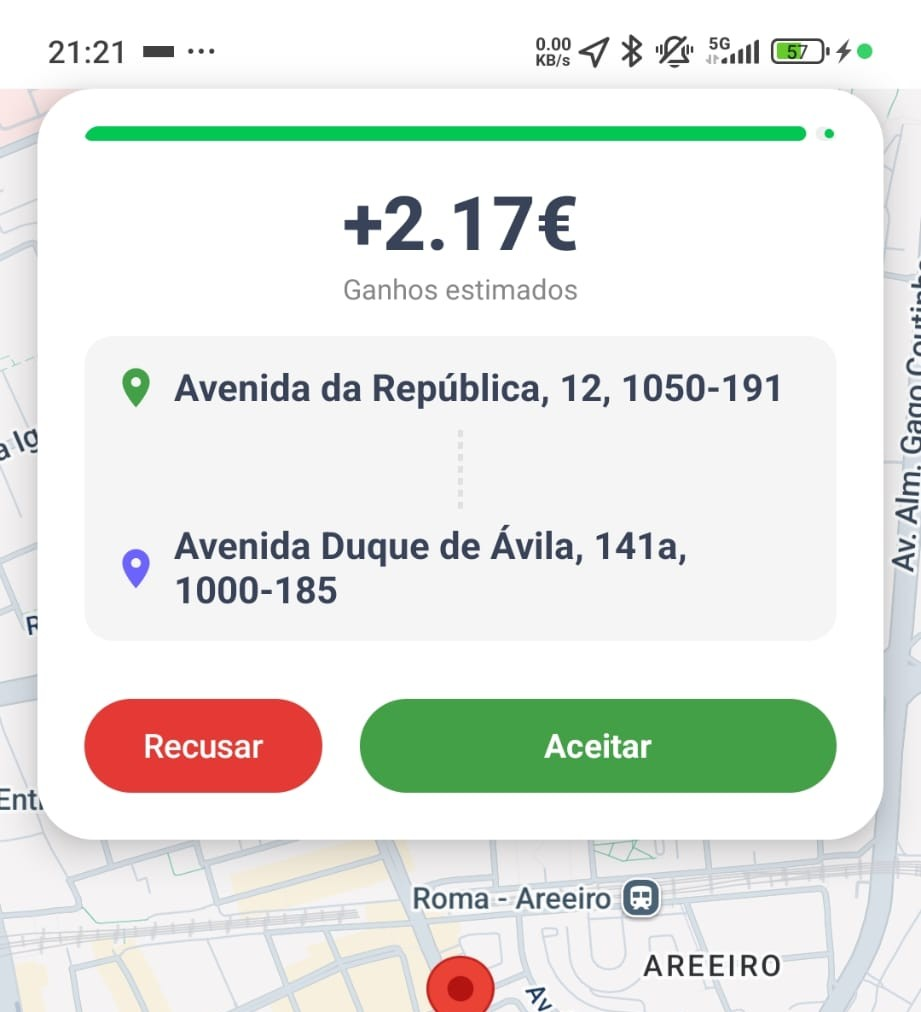
\includegraphics[width=\textwidth]{images/IncomingRequest.jpeg}
        \caption{Pickup confirmation screen}
        \label{fig:incoming_request}
    \end{subfigure}
    \hfill
    \begin{subfigure}[b]{0.48\textwidth}
        \centering
        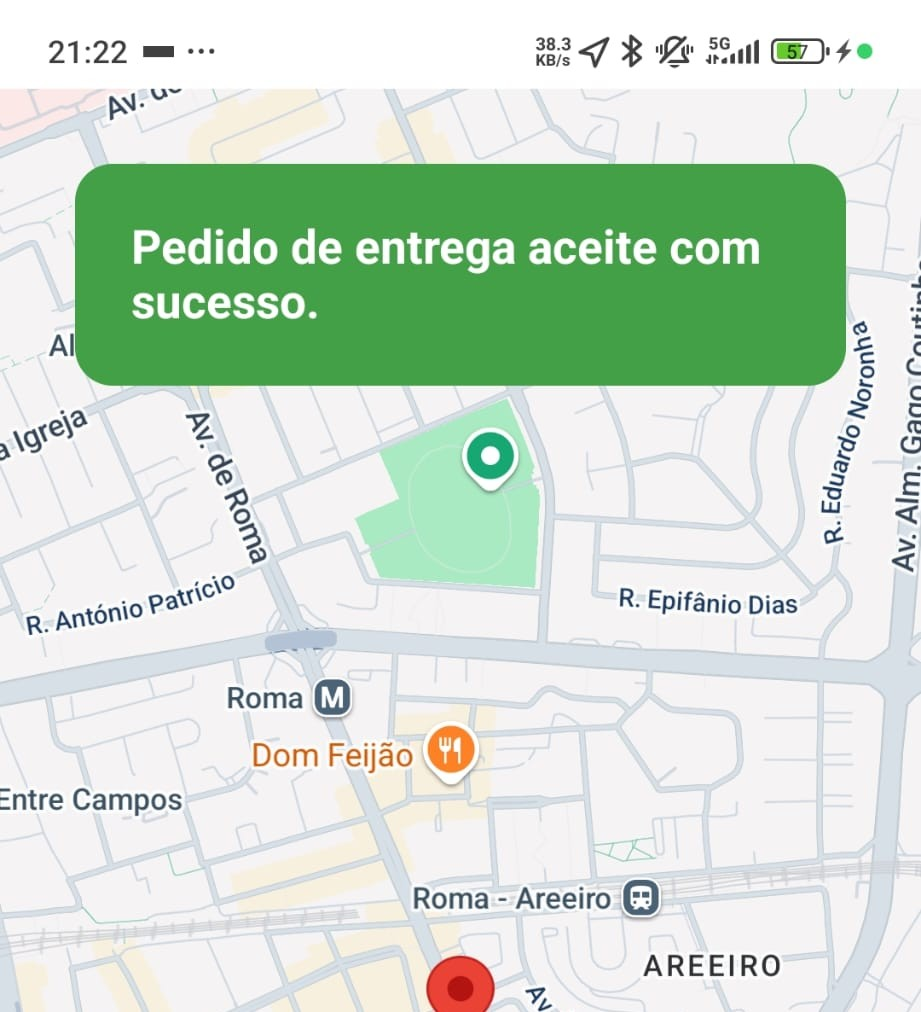
\includegraphics[width=\textwidth]{images/RequestAccepted.jpeg}
        \caption{Delivery confirmation screen}
        \label{fig:request_accepted}
    \end{subfigure}
    
    \vspace{0.5cm} % Slightly less space between rows
    
    \begin{subfigure}[b]{0.48\textwidth}
        \centering
        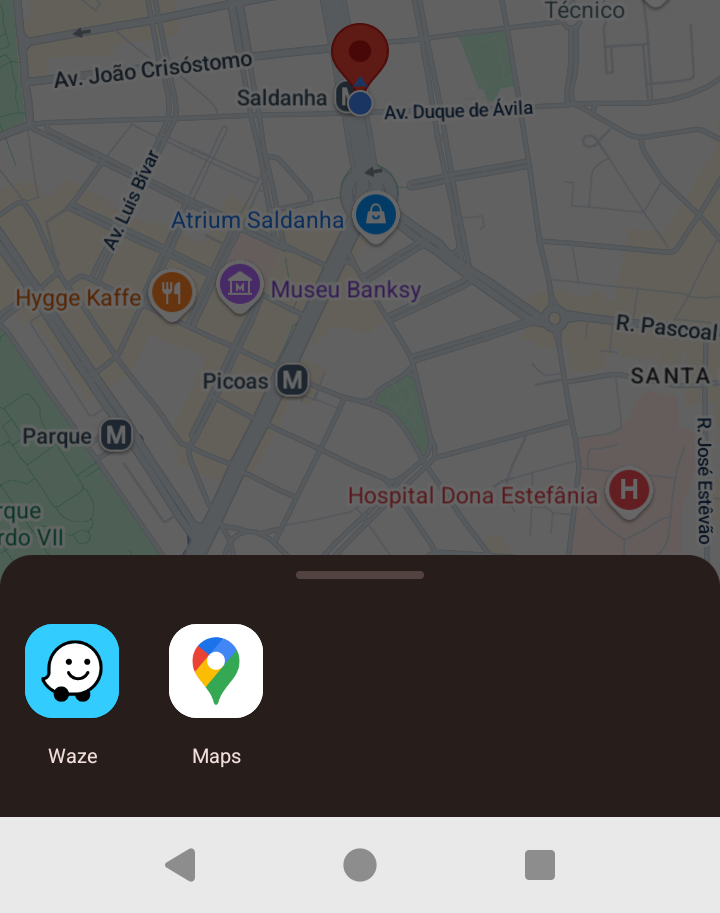
\includegraphics[width=\textwidth]{images/ChooseNavigationTool.png}
        \caption{Choose Navigation Tool}
        \label{fig:navigation_tool}
    \end{subfigure}
    \caption{Screens for confirming pickup, delivery and preferred navigation application choice }
    \label{fig:courier_request_accepted}
\end{figure}

\newpage

\subsubsection{Pickup and Drop-off Code Validation}

As part of the delivery confirmation flow, LiftDrop includes a code-based verification step to ensure that orders are only picked up or delivered by the correct courier. When a courier reaches the pickup or drop-off location, they can slide to pickup or dropoff the order.

This verification screen is shown only when the courier is sufficiently near the designated location (within 100 meters). If the provided code matches the one stored in the backend for that delivery, the delivery status proceeds to the next phase. Otherwise, an error state is triggered, and the user is prompted to retry.

\begin{figure}[H]
    \begin{subfigure}[b]{0.43\textwidth}
        \centering
        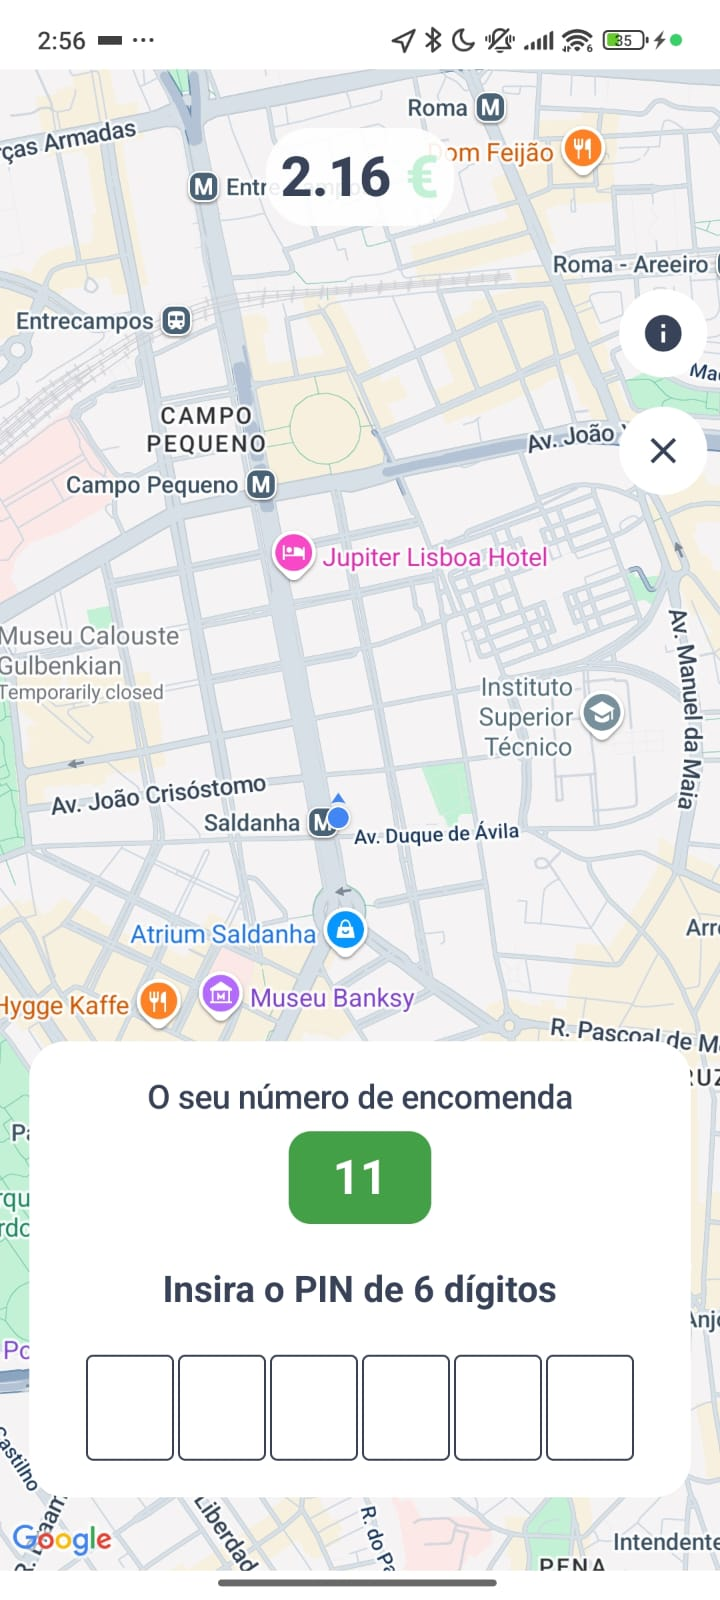
\includegraphics[width=\textwidth]{images/pickup_pin_screen.jpeg}
        \caption{Code entry screen for validating pickup or drop-off}
    \label{fig:code-verification}
    \end{subfigure}
    \hfill
    \begin{subfigure}[b]{0.43\textwidth}
        \centering
        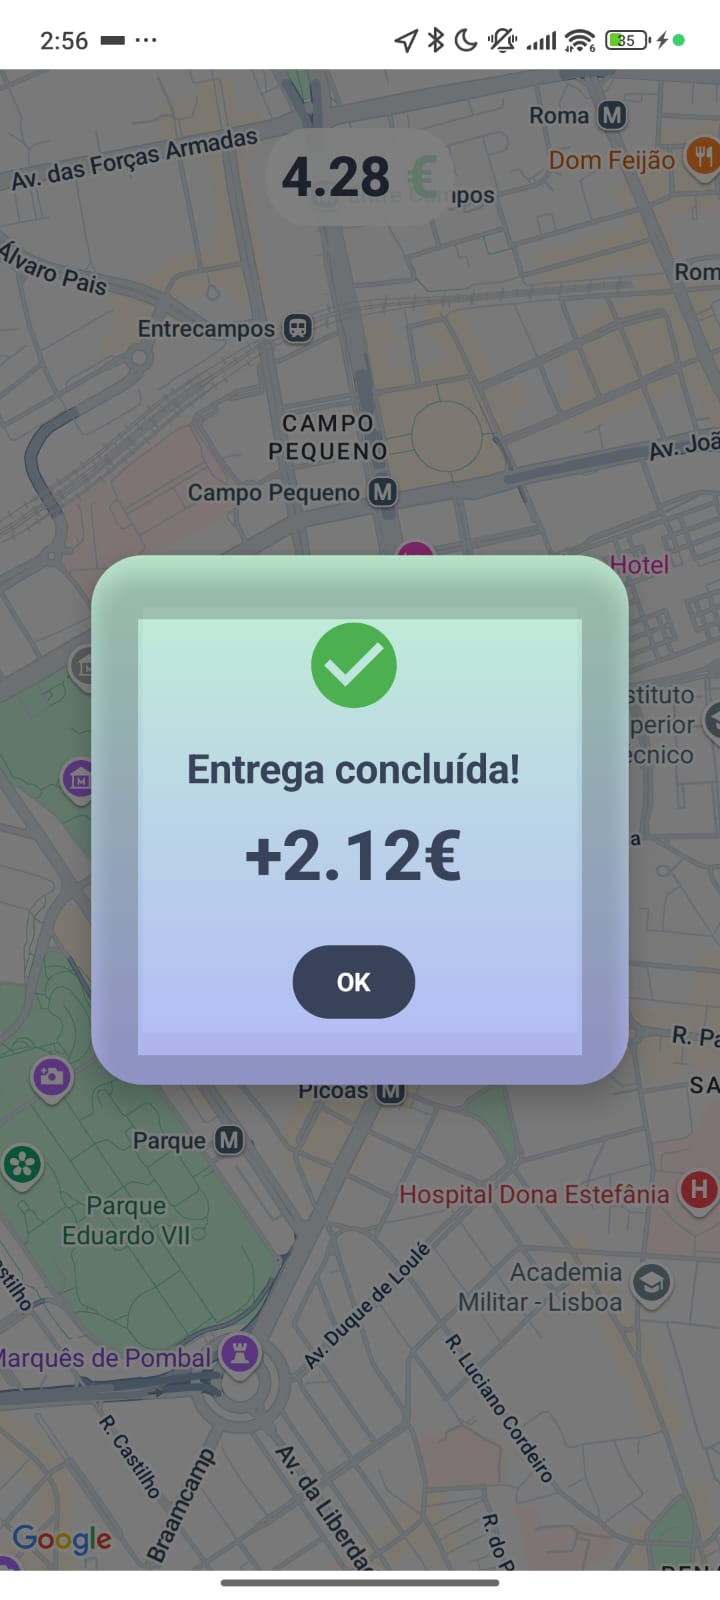
\includegraphics[width=\textwidth]{images/delivery_finished.jpeg}
        \caption{Delivery confirmation screen}
        \label{fig:delivery-finished}
    \end{subfigure}
\end{figure}

\newpage

\subsubsection{State Recovery and Rollback Mechanism}

To improve user experience and reduce friction after transient failures, the application implements a rollback strategy using a dedicated \texttt{previousState} flow. Before transitioning to an \texttt{Error} state, the ViewModel stores the current screen state in \texttt{previousState}.

If the user dismisses the error the app can safely restore the previous state by re-emitting its value into the main \texttt{stateFlow}. This ensures that the user returns to their previous workflow without losing context.

The mechanism is encapsulated in a small utility function responsible for managing both state transitions and error-aware rollbacks. We initially considered using this function for all state transitions to ensure consistent tracking of previous states across the application. However, this strategy proved unreliable in practice. Due to asynchronous coroutine scheduling and recomposition timing within the ViewModel scope, the function occasionally recorded stale or incorrect state values—particularly when multiple updates occurred in quick succession. 
To avoid introducing inconsistencies, we chose to restrict its use to fallback branches and error-handling paths (such as \texttt{else} clauses), where the current state is more stable and less likely to conflict with concurrent updates.

The helper function used for this purpose is shown below:

\begin{lstlisting}[language=Kotlin, caption={Safely updating screen state with rollback support}]
fun updateState(newState: HomeScreenState): HomeScreenState {
        // Salva o estado anterior
        _previousState.value = _stateFlow.value
        // Atualiza o estado atual
        _stateFlow.value = newState 
        return newState 
    }
\end{lstlisting}


\subsubsection{Persistent Local Storage with DataStore}

To persist authentication and user-specific data across sessions, LiftDrop uses Jetpack's \texttt{PreferencesDataStore}, a modern, coroutine-based alternative to \texttt{SharedPreferences}. It provides a lightweight and lifecycle-aware solution for storing key-value data such as the courier's ID, username, email, and bearer token.

These values are required to initiate authenticated requests and resume background services like location tracking. By storing them locally, the application can restore the session on cold start, reducing user friction and enabling seamless continuity.
The snippet below illustrates how the stored data is retrieved and reconstructed into a \texttt{UserInfo} object:


\begin{lstlisting}[language=Kotlin, caption={Retrieving stored user data from PreferencesDataStore}]
class PreferencesDataStore(
    private val store: DataStore<Preferences>
) : PreferencesRepository {
override suspend fun getUserInfo(): UserInfo? {

    val preferences = store.data.first()
    val username = preferences[nameKey]
    val courierId = preferences[idKey]
    val token = preferences[tokenKey]
    val email = preferences[emailKey]
    
    return if (username != null && courierId != null && token != null && email != null) {
        UserInfo(
            id = courierId,
            username = username,
            email = email,
            bearer = token,
        )
    } else null
} }
\end{lstlisting}

The \texttt{PreferencesRepository} interface is injected into the application through a central \texttt{DependenciesContainer}, as shown below. This allows the ViewModel and service layers to access user preferences in a decoupled and testable way.


\begin{lstlisting}[language=Kotlin, caption={Injecting PreferencesDataStore via DependenciesContainer}]
interface DependenciesContainer {
    val preferencesRepository: PreferencesRepository
    // Other services...
}

override val preferencesRepository: PreferencesRepository
    get() = PreferencesDataStore(dataStore)
\end{lstlisting}

\subsubsection{Frontend HTTP Service Abstraction}

While WebSocket communication powers real-time interactions between the courier and backend, the LiftDrop mobile application also relies on traditional HTTP requests for several operations, including authentication, data retrieval, and user profile updates.

To manage these requests consistently, a custom \texttt{HttpService} abstraction was implemented. This service is built on top of the \texttt{OkHttpClient} library, which provides a robust and efficient way to perform network operations on Android.

The \texttt{HttpService} encapsulates the logic for performing \texttt{GET}, \texttt{POST}, and \texttt{DELETE} requests, including header configuration, exception handling, and response parsing using Gson. Each method returns a unified result wrapper, allowing higher layers of the application to react appropriately to both successful and failed operations.

This design helps enforce separation of concerns while providing coroutine-compatible, type-safe methods for backend communication.

The following snippet shows the main structure of the \texttt{HttpService} class:

\begin{lstlisting}[language=Kotlin, caption={Frontend HttpService class for coroutine-based requests}]
class HttpService(
    val baseUrl: String,
    val client: OkHttpClient,
    val gson: Gson
) {
    suspend inline fun <reified T> get(url: String, token: String): Result<T> { ... }

    suspend inline fun <reified T, reified R> post(url: String, data: T, token: String): Result<R> { ... }

    suspend inline fun <reified T> delete(url: String, token: String): Result<T> { ... }
}
\end{lstlisting}

Each HTTP method in \texttt{HttpService} returns a sealed \texttt{Result} type, which standardizes how success and error outcomes are represented across the application. This abstraction allows ViewModels to process backend responses in a consistent and type-safe manner.

The definition of the \texttt{Result} class is shown below:

\begin{lstlisting}[language=Kotlin, caption={Sealed Result class used for HTTP responses}]
sealed class Result<out T> {
    data class Success<out T>(val data: T) : Result<T>()
    data class Error(val problem: Problem) : Result<Nothing>()
}
\end{lstlisting}

\subsection{Order Assignment Logic}

Order assignment is based on:

\begin{itemize}
    \item \textbf{Proximity to Pickup}: Calculated using Google Maps Distance Matrix API to ensure routing reflects real travel time, not just straight-line distance.
    \item \textbf{Courier Rating}: Couriers with higher ratings receive slight prioritization when travel times are similar.
\end{itemize}

To rank couriers based on proximity to the pickup location, we apply a two-phase sorting approach.

In the first phase, we sort couriers by their direct (as-the-crow-flies) distance to the pickup spot using PostgreSQL's PostGIS extension. This allows us to efficiently compute geographical distances between coordinates within the database. The following snippet illustrates how this is implemented:

\begin{lstlisting}[language=Kotlin, caption={Ranking couriers by direct distance using PostgreSQL PostGIS extension}]
override fun getClosestCouriersAvailable(
        pickupLat: Double, // Pickup spot's latititude
        pickupLng: Double, // Pickup spot's longitude
        requestId: Int, // Request id
        maxDistance: Double, // Max distance to be considered
    ): List<CourierWithLocation> =
        handle.createQuery("""
            SELECT ..., -- Other courier attributes
                ST_Distance(  -- Direct distance using PostGIS
                    ST_SetSRID(ST_MakePoint(l.longitude, l.latitude), 4326)::geography,
                    ST_SetSRID(ST_MakePoint(:pickupLon, :pickupLat), 4326)::geography
                ) AS distance_meters
            FROM ... -- Joins Courier table with Location table where courier is available
            AND ... -- Checks if courier has already declined this specific request
            AND ST_Distance( -- Gets 5 closest couriers
                    ST_SetSRID(ST_MakePoint(l.longitude, l.latitude), 4326)::geography,
                    ST_SetSRID(ST_MakePoint(:pickupLon, :pickupLat), 4326)::geography
                ) < :maxDistance
            ORDER BY distance_meters
            LIMIT 5;
            """,
            ).bind(...).list()
\end{lstlisting}

\noindent Once we've filtered and sorted couriers by their direct distance, we proceed to the second phase, where we refine the ranking based on their estimated travel time.

This is achieved by using the Google Maps Distance Matrix API, which takes into account real-world road data and traffic conditions to provide more accurate travel times. The snippet below shows how we perform this step:

\begin{lstlisting}[language=Kotlin, caption={Ranking couriers by travel time using Google Maps API}]
private suspend fun rankCouriersByTravelTime(
    couriers: List<CourierWithLocation>,
    destinationLat: Double,
    destinationLon: Double,
): List<CourierWithLocation> {
    val origins = couriers.joinToString("|") { "${it.latitude},${it.longitude}" }
    val destination = "$destinationLat,$destinationLon"
    

    // Sends a request to the Google Maps Distance Matrix API,
    // using courier locations as origins and the destination as the drop-off point.
    val response = ...
    
    // Parses the API response to extract a list of travel times (in seconds), where each value corresponds to a courier in the original list.
    val travelTimes = ...

    // Combines each courier with their corresponding travel time,
    // sort them in ascending order of travel time,
    // and return a list of couriers with the estimated travel time included.
    return couriers.zip(travelTimes)
        .sortedBy { it.second }
        .map { (courier, time) -> courier.copy(estimatedTravelTime = time) }
}
\end{lstlisting}

After obtaining the estimated travel times, each courier is scored using a weighted formula that combines normalized travel time and user rating. Couriers with lower scores are ranked higher and prioritized for order assignment.

\begin{lstlisting}[language=Kotlin, caption={Scoring couriers by travel time and rating}]
fun rankCouriersByScore(couriers: List<CourierWithLocation>): List<CourierWithLocation> {
    val minTime = couriers.minOf { it.estimatedTravelTime ?: 0L }
    val maxTime = couriers.maxOf { it.estimatedTravelTime ?: 1L }
    val minRating = couriers.minOf { it.rating ?: 0.0 }
    val maxRating = couriers.maxOf { it.rating ?: 5.0 }

    val alpha = 0.7 // weight for travel time
    val beta = 0.3  // weight for rating

//Faster couriers and those with higher ratings get a lower score.
    return couriers.sortedBy { courier ->
        val normTime = if (maxTime > minTime) {
            ((courier.estimatedTravelTime ?: 0L) - minTime).toDouble() / (maxTime - minTime)
        } else 0.0

        val normRating = if (maxRating > minRating) {
            ((courier.rating ?: 0.0) - minRating) / (maxRating - minRating)
        } else 0.0

        alpha * normTime + beta * (1 - normRating)
    }
}
\end{lstlisting}

Lastly, the centerpiece of LiftDrop’s dynamic dispatching logic is the courier assignment handler, which orchestrates several previously discussed components into a single cohesive workflow. This function initiates the process of locating available couriers within an incrementally expanding search radius, sending them real-time assignment requests, and awaiting their responses. If a courier accepts, the assignment is confirmed; if not, the system proceeds to the next available candidate. This recursive mechanism ensures robust and flexible request fulfillment. The snippet below illustrates how these interconnected elements are brought together:


\begin{lstlisting}[language=Kotlin, caption={Handling Courier Assignments (Simplified Pseudocode)}]
suspend fun handleCourierAssignment(
    pickupLat: Double,
    pickupLon: Double,
    requestId: Int,
    currentMaxDistance: Double = 1000.0,
    maxDistanceIncrement: Double = 1000.0,
    maxAllowedDistance: Double = 4000.0,
    deliveryKind: String
): Boolean {

    if (currentMaxDistance > maxAllowedDistance) return false

    val couriers = fetchAvailableCouriers(pickupLat, pickupLon, currentMaxDistance, deliveryKind)

    if (couriers is Either.Right) {
        for (courier in couriers.value) {
            val response = AssignmentCoordinator.register(requestId)
            val accepted = transactionManager.run {
                val details = getRequestDetails(requestId)
                val earnings = estimateEarnings(details)
                WebSocketHandler.sendAssignmentMessageToCourier(courier.courierId, details)

                try {
                    withTimeout(20_000) { response.await() }
                } catch (_: TimeoutCancellationException) { false }
            }

            if (accepted) return true
            else WebSocketHandler.handleDecline(courier.courierId, requestId)
        }
    }

    delay(10_000)
    return handleCourierAssignment(
        pickupLat, pickupLon, requestId,
        currentMaxDistance + maxDistanceIncrement,
        maxDistanceIncrement,
        maxAllowedDistance,
        deliveryKind
    )
}

\end{lstlisting}



To facilitate asynchronous communication between the backend and couriers during the assignment process, the system leverages a dedicated coordination component named AssignmentCoordinator. This object maintains an in-memory registry that maps each delivery request ID to a corresponding \texttt{CompletableDeferred<Boolean>} instance. When a courier assignment is initiated, the request is registered and a deferred response is created. This deferred serves as a synchronization point, allowing the backend to suspend execution while awaiting the courier’s response. Once the courier accepts or declines the assignment, the complete function is invoked to resolve the deferred and resume the assignment logic accordingly. This mechanism enables non-blocking, thread-safe handling of real-time interactions in the courier dispatch workflow.

\vspace{5.0mm}

\begin{lstlisting}[language=Kotlin, caption={Assignment Coordination}]
object AssignmentCoordinator {
    private val pendingResponses = ConcurrentHashMap<Int, CompletableDeferred<Boolean>>()

    fun register(requestId: Int): CompletableDeferred<Boolean> {
        val deferred = CompletableDeferred<Boolean>()
        pendingResponses[requestId] = deferred
        return deferred
    }

    fun complete(
        requestId: Int,
        accepted: Boolean,
    ) {
        pendingResponses.remove(requestId)?.complete(accepted) ?: log("Already completed or missing")
    }
}
\end{lstlisting}

\newpage

\subsection{Canceling Orders}

Order cancellations were designed to be seamless. If a courier cancels before pickup, the system treats the order as unassigned and assigns it to nearby couriers. If cancellation occurs after pickup, the order is re-assigned using the courier’s last known location as the new pickup point. This design ensures minimal disruption to the overall system.
The following sketch illustrates the two possible user journeys when a courier cancels an order.

\begin{figure}[H]
    \centering
    \includegraphics[width=0.56\textwidth]{images/CourierCancelJourney.png}
    \caption{Courier Order Canceling Journey}
\end{figure}

\newpage

Before reassigning a canceled request, the system determines the appropriate pickup coordinates and pin code based on the current delivery status. If the request was canceled after pickup, a message is sent to the canceling courier to retrieve the pin code. This pin code is then passed along to the newly assigned courier to ensure the delivery can still be completed securely.

\begin{lstlisting}[language=Kotlin, caption={Reassignment of a cancelled request}]
fun handleRequestReassignment(
        requestId: Int,
        courierId: Int,
        deliveryStatus: DeliveryStatus,
        pickupLocationDTO: LocationDTO?,
    ): Boolean {
        return transactionManager.run {
            ... // pickupLat, pickupLon and pickupPin are determined according to the delivery status

            CoroutineScope(Dispatchers.Default).launch {
                if (handleCourierAssignment(
                        pickupLat = pickupLat,
                        pickupLon = pickupLon,
                        requestId = requestId,
                        deliveryKind = deliveryStatus.toDeliveryKind().name,
                    )
                ) {
                    if (deliveryStatus == DeliveryStatus.HEADING_TO_DROPOFF) {
                        courierWebSocketHandler.sendMessageToCourier(
                            courierId = courierId,
                            message =
                                DeliveryUpdateMessage(
                                    hasBeenAccepted = true,
                                    pinCode = pickupPin
                                ),
                        )
                    } else {
                        GlobalLogger.log("Courier $courierId reassigned to request $requestId")
                    }
                }
            }
            return@run true
        }
    }
\end{lstlisting}

\vspace{5mm}

The following can be observed when that happens in the following figures:

\begin{figure}[H]
    \centering
    % First row
    \begin{subfigure}[b]{0.47\textwidth}
        \centering
        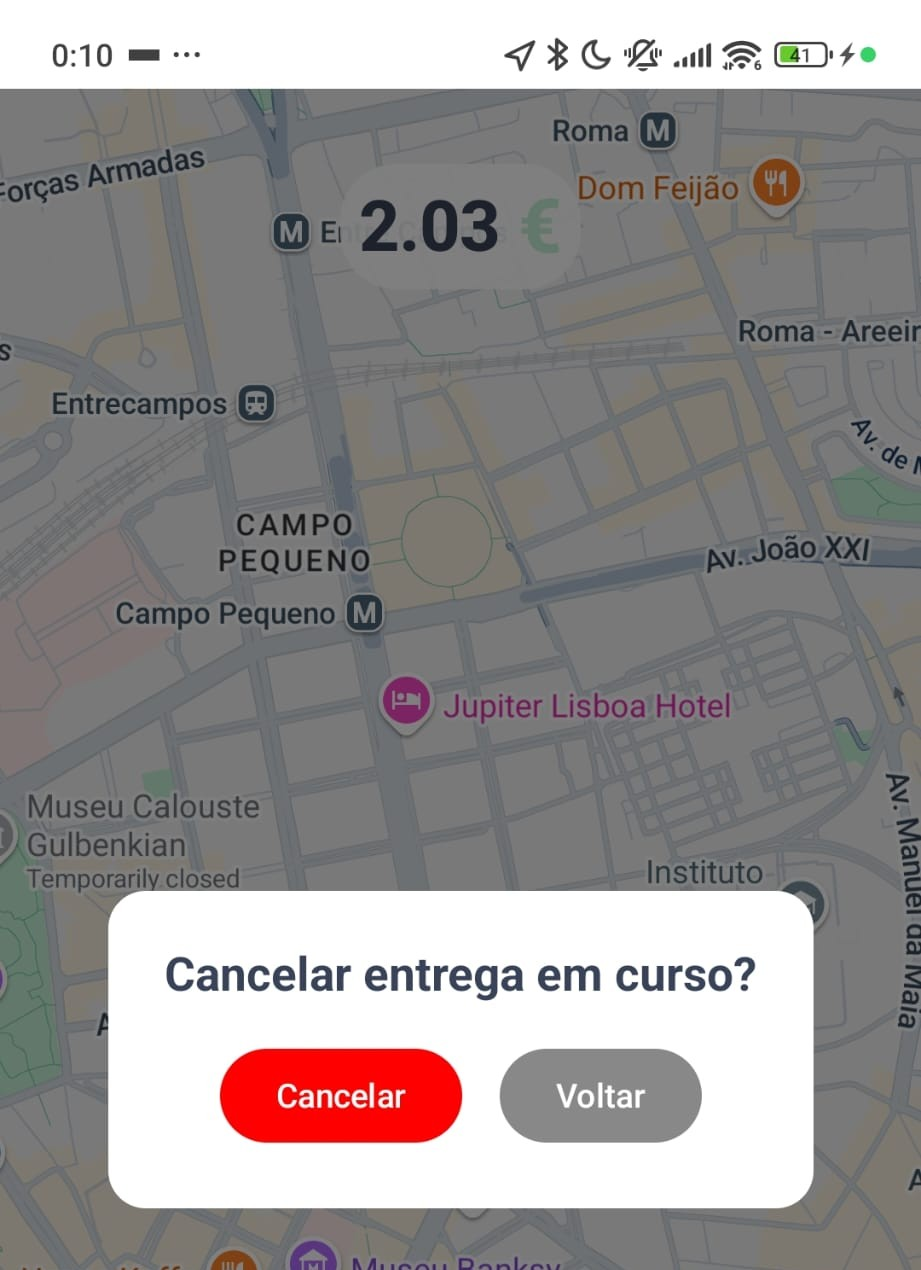
\includegraphics[width=\textwidth]{images/CancelConfirmation.jpeg}
        \caption{Cancel confirmation screen}
        \label{fig:cancel_confirmation}
    \end{subfigure}
    \hfill
    \begin{subfigure}[b]{0.47\textwidth}
        \centering
        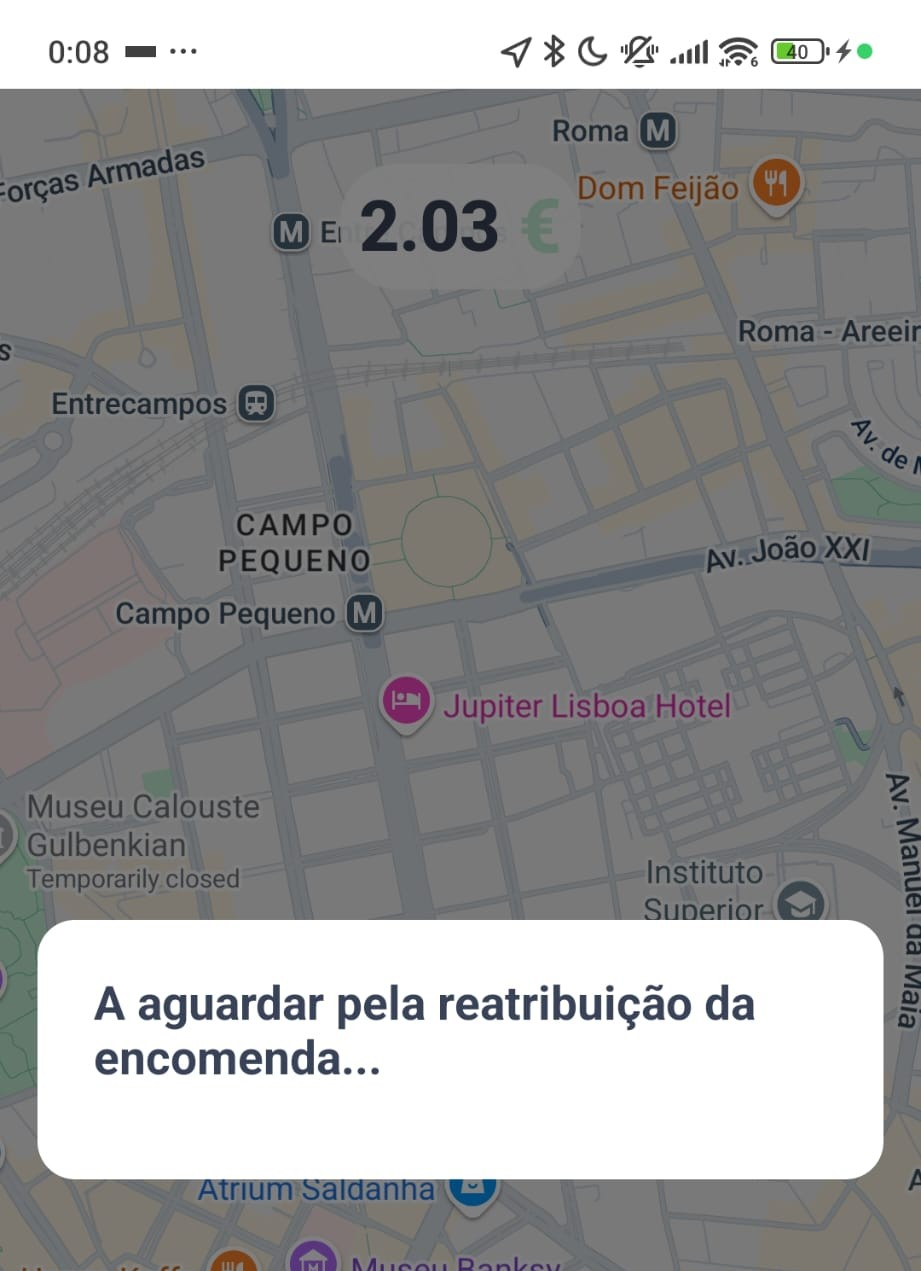
\includegraphics[width=\textwidth]{images/CancelReassignment.jpeg}
        \caption{Reassignment in progress screen}
        \label{fig:cancel_reassignment}
    \end{subfigure}
    
    \vspace{0.3cm} % Slightly less space between rows

    % Second row
    \begin{subfigure}[b]{0.47\textwidth}
        \centering
        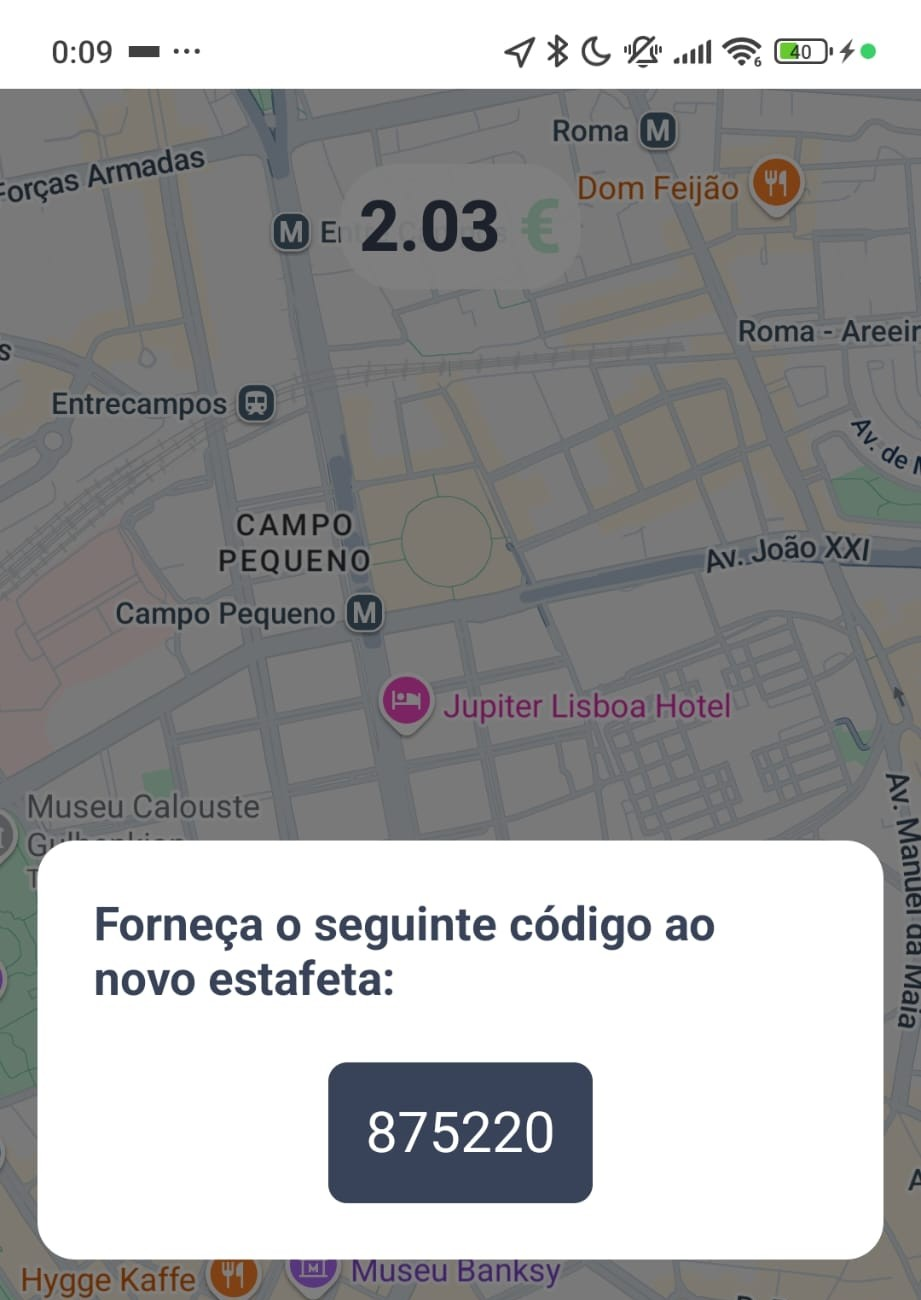
\includegraphics[width=\textwidth]{images/CodeReassignment.jpeg}
        \caption{Pickup code for reassigned courier}
        \label{fig:code_reassignment}
    \end{subfigure}
    \hfill
    \begin{subfigure}[b]{0.47\textwidth}
        \centering
        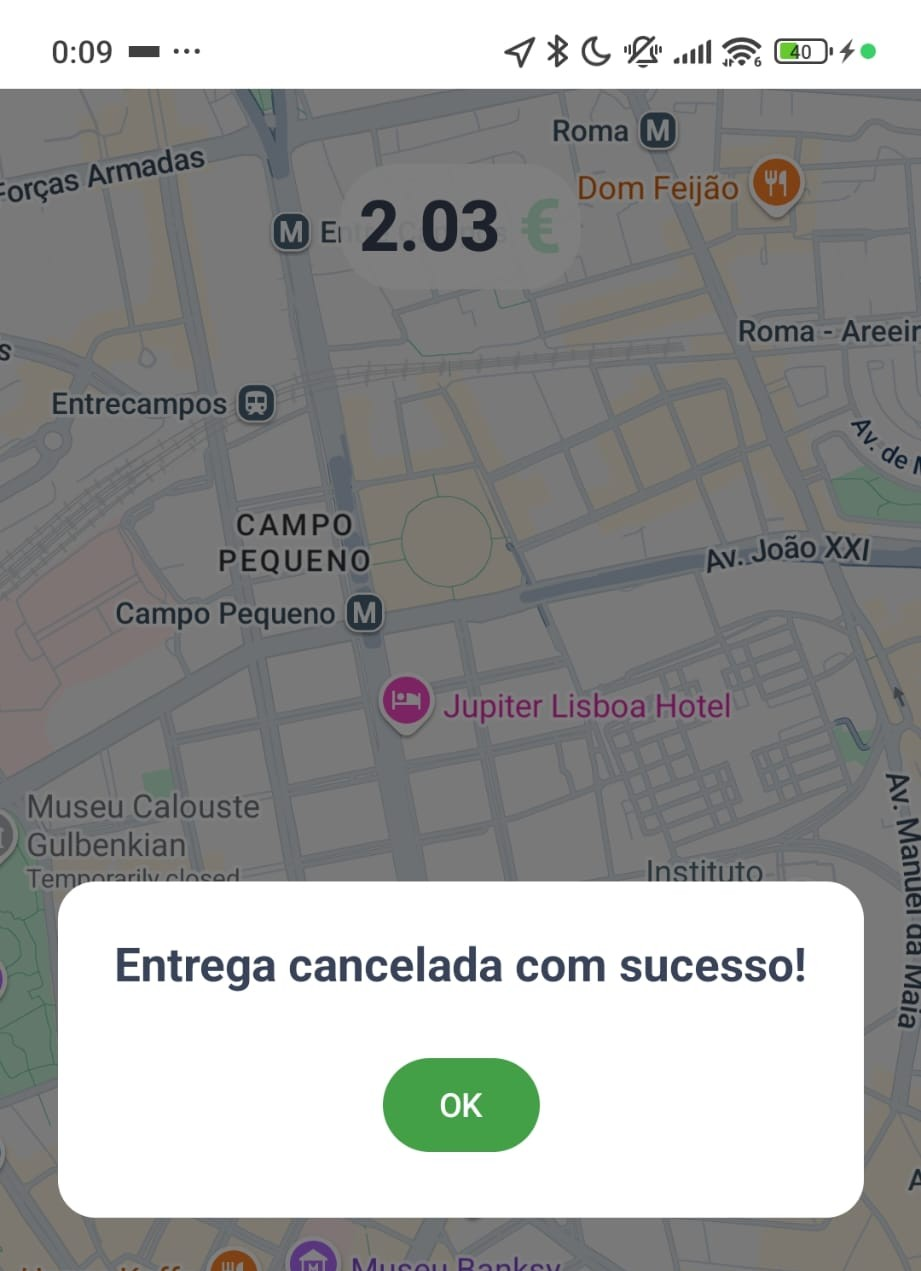
\includegraphics[width=\textwidth]{images/CancelSuccess.jpeg}
        \caption{Successful cancellation confirmation}
        \label{fig:cancel_success}
    \end{subfigure}

    \caption{UI states for order cancellation and reassignment flow}
    \label{fig:cancel_and_reassign_flow}
\end{figure}

\newpage

\subsection{Courier Earnings}

LiftDrop calculates courier earnings using a mix of fixed and dynamic components:

\begin{itemize}
    \item \textbf{Base Fee}: A flat fee for completing any order.
    \item \textbf{Distance Fee}: A per-kilometer rate based on travel distance from courier to pickup.
    \item \textbf{Item Value Multiplier}: A bonus based on order value to reflect risk or effort for higher-priced deliveries.
    \item \textbf{Quantity}: All components are scaled by the number of items in the delivery.
\end{itemize}

\noindent The Kotlin function below shows the earnings calculation:

\begin{lstlisting}[language=Kotlin, caption={Calculation of Courier Earnings}]
fun estimateCourierEarnings(
        distanceKm: Double,
        itemValue: Double,
        quantity: Int,
        baseFee: Double = 2.0,
        perKmRate: Double = 0.5,
        valueRate: Double = 0.005,
    ): Double = quantity * (baseFee + (distanceKm * perKmRate) + (itemValue * valueRate))
\end{lstlisting}

\subsection{Database Access}

The LiftDrop backend interacts with the PostgreSQL database through a transactional abstraction based on JDBI. The design separates transaction management from repository implementation, ensuring consistency and maintainability across all database operations.

The following Kotlin class handles transactional execution using JDBI:

\begin{lstlisting}[language=Kotlin, caption={JDBI Transaction Manager}]
@Component
class JdbiTransactionManager(
    private val jdbi: Jdbi,
) : TransactionManager {
    override fun <R> run(block: (Transaction) -> R): R =
        jdbi.inTransaction<R, Exception> { handle ->
            val transaction = JdbiTransaction(handle)
            block(transaction)
        }
}
\end{lstlisting}

The `JdbiTransaction` class exposes repository instances tied to the same underlying handle, allowing atomic operations across multiple tables:

\begin{lstlisting}[language=Kotlin, caption={JDBI Transaction with Repository Bindings}]
class JdbiTransaction(
    private val handle: Handle,
) : Transaction {
    override val usersRepository = JdbiUserRepository(handle)
    override val clientRepository = JdbiClientRepository(handle)
    override val requestRepository = JdbiRequestRepository(handle)
    override val courierRepository = JdbiCourierRepository(handle)
    override val deliveryRepository = JdbiDeliveryRepository(handle)
    override val locationRepository = JdbiLocationRepository(handle)
}
\end{lstlisting}

This architecture enables consistent, testable, and atomic data operations while maintaining separation of concerns between business logic and persistence logic.

\subsection{Tests}

The LiftDrop platform was tested through both manual and automated approaches to ensure correctness, reliability, and performance. Testing focused on backend behavior, including API functionality, business logic, and role-based access control.

\subsubsection{Manual Tests}

Manual tests were primarily used to verify API behavior and end-to-end interactions between clients and couriers. These tests were executed using \textbf{Postman}, allowing us to simulate real HTTP requests and observe responses in real time.

Key scenarios tested manually included:
\begin{itemize}
    \item User registration and authentication
    \item Order creation and assignment
    \item Role-based access restrictions
    \item Session persistence via cookies
    \item Order cancellation and reassignment
\end{itemize}

\subsubsection{Automated Tests}

Automatic tests were written using the \textbf{JUnit} testing framework to validate the backend’s core business logic. These tests were executed during development to catch regressions and verify key modules in isolation.

Test coverage included:
\begin{itemize}
    \item Unit tests for repositories and services
    \item Validation of order assignment logic
    \item Verification of courier scoring algorithms
    \item Authentication and authorization checks
\end{itemize}

In future iterations, these tests can be extended with integration and UI testing using tools like Espresso or Retrofit mock services.


